\begin{filecontents*}{\jobname.xmpdata}
    \Title     {Atividade 07 - Triangulação de Delauney}
    \Author    {João Pedro Rosa Cezarino}
    \Keywords  {CC6112\sep OpenGL\sep Cameras\sep FEI}
    \Language  {pt-BR}
    \Subject   {Resolução da Atividade 07 - Triangulação de Delauney - CC6112}
\end{filecontents*}

\documentclass[a4paper, 12pt]{article}
\usepackage[utf8]{inputenc}
\usepackage[bottom=3cm,top=2.5cm,left=2cm,right=2cm]{geometry}
\usepackage[brazil]{babel}
\usepackage{graphicx} 
\usepackage{amsmath}
\usepackage{amssymb}
\usepackage{fancyhdr}
\usepackage{xcolor}
\fancyhf{}
\pagestyle{fancy}
\fancyfoot[LE,RO]{\thepage}
\setlength\headheight{26pt}
\rhead{
\includegraphics[width=4cm]{template-FEI/FEI_logo.png}}

\begin{document}
\noindent \textbf{Centro Universitário FEI}\\
\noindent \textbf{CC6112 - Computação Gráfica}\\
\noindent \textbf{Aluno: } Thales Lacerda de Oliveira  \\ 
\noindent \textbf{R.A: } 22.120.021-5\\
\today
\\
\begin{center}
    \noindent \textbf{Resolução da Atividade 07 - Triangulação de Delauney}
\end{center}

\vspace{0.5cm}
\noindent\textbf{Questão 01:}\\
Defina de maneira informal o que é uma Malha Triangular. Exemplos: \emph{(1)} se fosse
perguntado, defina o que é um quadrado, a resposta poderia ser: Um quadrado é um
conjunto de quatro pontos, onde cada ponto é vizinho de outros três, mas é ligado por
arestas apenas a seus dois vizinhos mais próximos. Além disso, as distâncias entre esses
dois vizinhos mais próximos são as mesmas. \emph{(2)} se fosse perguntado o que é um triângulo,
a resposta poderia ser: Um triângulo é um conjunto de três pontos, todos ligados entre si
por arestas.\\
\\
\noindent\textbf{Solução:}\\
Uma Malha Triangular é uma malha onde todo conjunto de três vértices vizinhos se conectam formando um triângulo. Além disso, a cada 3 pontos conectados, não deve existir cruzamento entre as arestas.
\vspace{0.7cm}

\noindent\textbf{Questão 02:}\\
Defina de maneira informal o que é a Malha de Delauney.\\
\\
\noindent\textbf{Solução:}\\
A Malha de Delauney é a malha com a melhor triangularização encontrada, ou seja, uma malha onde a ordem lexicográfica é máxima. A triangulação é perfeita se, e somente se, o Flip de qualquer aresta deixar a triangularização pior.
\vspace{0.7cm}

\noindent\textbf{Questão 03:}\\
Defina, formalmente, o que é Malha de Delauney. OBS: existem algumas exemplos de
definições formais nos vídeos e materiais no Moodle.\\
\\
\noindent\textbf{Solução:}\\
Uma triangulação T de P é dita ser de Delauney se, para qualquer outra triangulação $\mathbf{T'}$ e $\mathbf{P}$ \rightarrow $A(T) \geq A(T')$. Onde $\mathbf{A}$ é o vetor de ângulos de T.
\vspace{0.7cm}

\noindent\textbf{Questão 04:}\\
Em que princípio que se baseia a triangulação de Delauney para ser considerada a
melhor? Para responder essa pergunta, note que “princípio” é uma verdade subjetiva,
que pode ser contrariada.\\
\\
\noindent\textbf{Solução:}\\
Para a Triangulação de Delauney ser considerada a melhor, utiliza-se o princípio de que quanto mais obtuso for o ângulo, melhor é a ordem lexicográfica e, por consequência, melhor é a malha.
\vspace{1cm}

\noindent\textbf{Questão 05:}\\
A Figura 1 a seguir mostra uma sequência de quadros onde, em cada um, estão
sendo adicionados pontos da Triangulação de Delauney. Cada quadro
corresponde à adição de um único ponto. Essa sequência deve ser observada da
direita para a esquerda e de cima pra baixo. Para cada quadro, você deve
completar as arestas que são criadas. Considere que não há necessidade de flipar
nenhuma aresta adicionada.\\
\\
\noindent\textbf{Solução:}\\
\begin{center}
    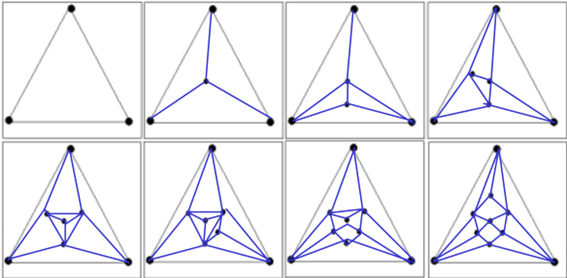
\includegraphics[width=13cm,height=6cm]{img_01.png}
\end{center}
\vspace{1cm}

\noindent\textbf{Questão 06:}\\
Para a questão 5, mostre a árvore final que guarda a triangulação construída.\\
\\
\noindent\textbf{Solução:}\\
\begin{center}
    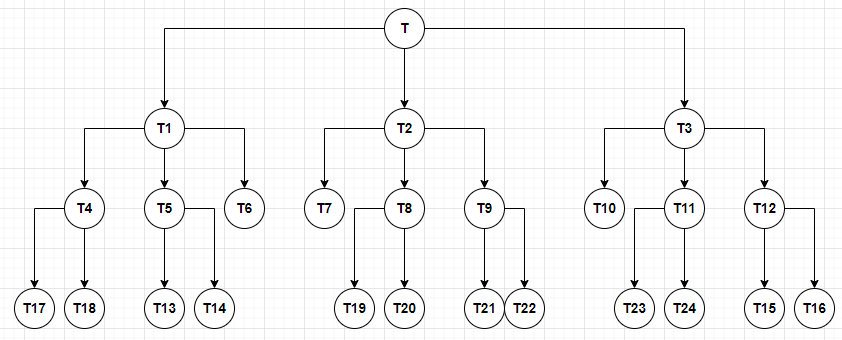
\includegraphics[width=14cm,height=7cm]{img_02.png}
\end{center}
\newpage

\noindent\textbf{Questão 07:}\\
Mostre o Pseudocódigo do Algoritmo de Triangulação de Delaunay visto em
sala.\\
\\
\noindent\textbf{Solução:}
\begin{center}
    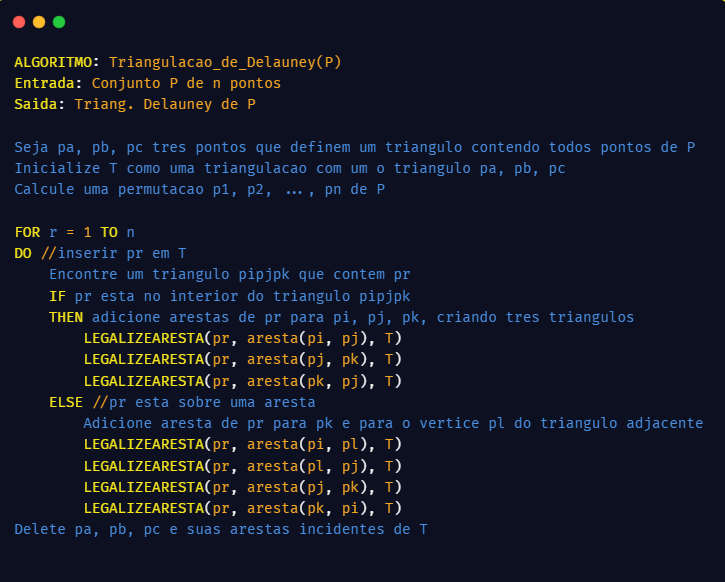
\includegraphics[width=13cm,height=10cm]{img_03.png}
\end{center}
\vspace{0.2cm}

\noindent\textbf{Questão 08:}\\
Seja a distribuição de um conjunto de pontos no plano (Figura 2 a seguir) durante a
execução do algoritmo de triangulação de Delaunay, visto em sala (reproduzido a seguir)
imediatamente após a inserção do ponto P1 e imediatamente antes das chamadas das
rotinas de legalização de arestas.\\
\\
\noindent\textbf{Solução:}\\
\noindent\text{Antes da legalização:}
\begin{center}
    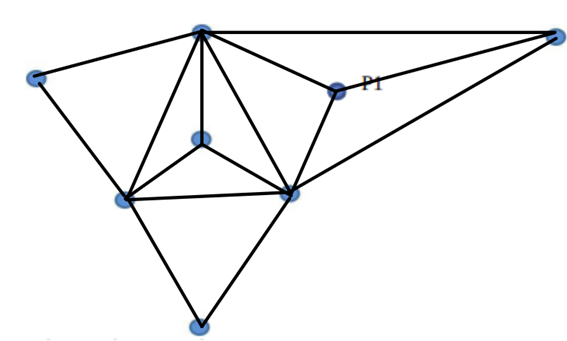
\includegraphics[width=9cm,height=7cm]{img_04.png}
\end{center}
\noindent\text{Depois da legalização:}
\begin{center}
    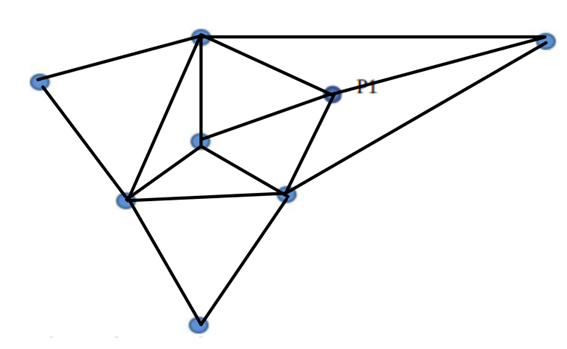
\includegraphics[width=9cm,height=7cm]{img_05.png}
\end{center}
\vspace{1.0cm}

\noindent\textbf{Questão 09:}\\
No algoritmo de construção de malhas \emph{3D} utilizando a triangulação de Delauney (dado
em sala), existem duas situações distintas e importantes que são destacadas pelo
algoritmo. A primeira, um vértice \textbf{pr} pode cair sobre uma aresta e, ligada a vértices \textbf{pi},\textbf{pj}.Nesse caso, e é uma aresta oposta a vértices \textbf{pkpl}. Na segunda, pr cai dentro do triângulo formado pelas arestas \textbf{pi}, \textbf{pj}, \textbf{pk}. Explique, utilizando a notação dada, quais as ações tomadas pelo algoritmo em cada situação.\\
\\
\noindent\textbf{Solução:}\\
\\
Caso o vértice \textbf{pr} caia dentro do triângulo formado pelas arestas \textbf{pi, pj, pk}, o algoritmo vai criar 3 novos triângulos, filhos de \textbf{pr} e deve-se flipar as arestas opostas à \textbf{pr}, para manter a ordem lexicográfica crescente:
\begin{itemize}
    \item \textbf{LEGALIZEARESTA}(pr, aresta (pi, pj), T)
    \item \textbf{LEGALIZEARESTA}(pr, aresta (pj, pk), T)
    \item \textbf{LEGALIZEARESTA}(pr, aresta (pk, pi), T)
\end{itemize}
Se o vértice \textbf{pr} cair sobre uma aresta já existente, remove-se a aresta onde \textbf{pr} caiu, criam-se 4 novos triângulos filhos e por fim, flipam-se as arestas para manter a ordem lexicográfica crescente e a triangulação perfeita.
\begin{itemize}
    \item \textbf{LEGALIZEARESTA}(pr, aresta (pi, pl), T)
    \item \textbf{LEGALIZEARESTA}(pr, aresta (pl, pj), T)
    \item \textbf{LEGALIZEARESTA}(pr, aresta (pj, pk), T)
    \item \textbf{LEGALIZEARESTA}(pr, aresta (pk, pi), T)
\end{itemize}
\vspace{1cm}

\noindent\textbf{Questão 10:}\\
A malha triangular da Figura 1 mostra o momento em que os pontos \emph{P1} a \emph{P5} acabaram de
ser inseridos e as arestas já foram adequadamente “flipadas”. Em seguida, foi adicionado
o ponto \emph{P6}, que, ao ser ligado aos pontos \emph{P3}, \emph{P2} e \emph{P4}, os divide os ângulos $\alpha4$, $\alpha5$ e $\alpha6$ exatamente em suas metades. Sabe-se que uma aresta de \emph{P6} a \emph{P1} divide $\alpha1$ também na metade, e o mesmo acontece com $\alpha9$ quando ligamos \emph{P6} a \emph{P5}. Sabendo-se que esses ângulos são: $\alpha1$, $\alpha2$, $\alpha3$, $\alpha4$, $\alpha5$, $\alpha6$, $\alpha7$, $\alpha8$, $\alpha9$ = {90, 30, 60, 60, 30, 90, 40, 60, 80}, respectivamente, de acordo com o princípio de Delauney, faça o desenho de como ficaria a configuração final da malha.\\
\\
\noindent\textbf{Solução:}\\
\begin{center}
    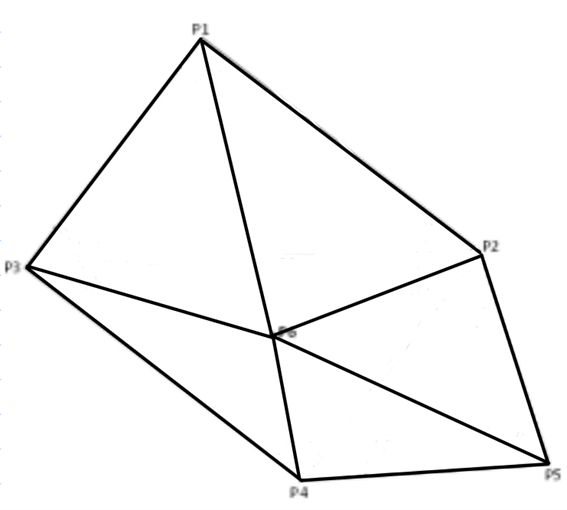
\includegraphics[width=10cm,height=8cm]{img_06.png}
\end{center}
\vspace{1cm}

\noindent\textbf{Questão 11:}\\
Mostre um exemplo em que o princípio da aplicação da ordem lexicográfica crescente
falha, e a malha resultante no Algoritmo de Delauney não estaria correto.
\\
\\
\noindent\textbf{Solução:}\\
\begin{center}
    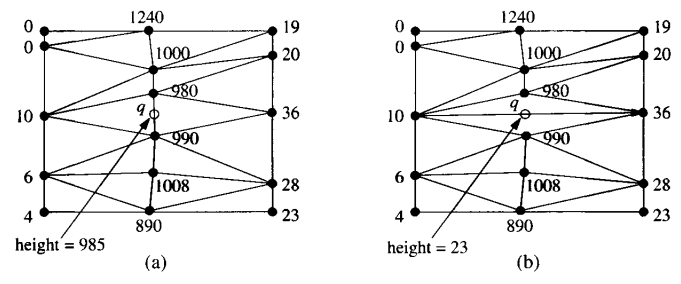
\includegraphics[]{img_07.png}
\end{center}
Através do exemplo acima, verifica-se que, apesar de a primeira imagem estar de acordo com o algoritmo de Delauney, não podemos garantir que ela é melhor que a segunda imagem, uma vez que a altura entre os pontos 980 e 990 é menor no segundo caso, onde os ângulos são pequenos.
\vspace{1cm}

\noindent\textbf{Questão 12:}\\
Imagine que você tem uma Malha de Delauney com $\mathbf{N = 10^k}$ pontos, onde \emph{k} é um número
inteiro muito grande, e você precisa varrer a malha para encontrar um ponto específico
que deseja calcular a intensidade de iluminação. Qual é a ordem de complexidade, no
pior caso, da busca por esse ponto?
\\
\\
\noindent\textbf{Solução:}\\
A ordem de complexidade da busca por este ponto, no pior caso, seria de: $\mathbf{\log_3 n}$. Já que, cada ponto colocado na malha geraria 3 novos triângulos, no pior caso.
\vspace{1cm}

\end{document}

